\documentclass[11pt]{article}
\usepackage[margin=1in]{geometry}
\usepackage[T1]{fontenc}
\usepackage{lmodern,microtype,amsmath,amssymb,amsthm,booktabs,graphicx}
\usepackage{xcolor}
\usepackage[colorlinks=true,linkcolor=blue!45!black,citecolor=blue!45!black,urlcolor=blue!45!black]{hyperref}
\usepackage{enumitem}
\setlist{itemsep=2pt,topsep=4pt}
\newtheorem{proposition}{Proposition}
\newtheorem{corollary}{Corollary}
\newcommand{\Hh}{\mathcal H}
\newcommand{\Paths}{\mathcal P}
\newcommand{\dd}{\,\mathrm d}
\title{Delayed departure can reverse the exposure benefit\\of a mine escape connection}
\author{}
\date{Working preprint --- October 25, 2026}
\begin{document}
\maketitle
\begin{abstract}
An additional tunnel gives evacuees more route choices, but also gives floodwater another route. Can the same connection reduce flood exposure for an early evacuee and increase it for a late evacuee, even when each chooses the best available route? We construct a low-lying tunnel-network motif in which this reversal occurs under two different hydraulic models. An added connection initially diverts water away from an existing escape route, then feeds accumulation at the worker's origin. A simple origin-depth lower bound certifies late harm independently of route optimization: the worker already encounters more water at departure than an explicit escape trajectory encounters anywhere in the original layout. In a locally frozen 16-condition factorial, 12 conditions meet a prespecified 2\,cm early-benefit/late-harm criterion in both models. All 16 admit the late-harm certificate in both models at three walking speeds. Refinement, junction-storage changes, and depth-responsive walking preserve the sign in the tested cases, although not every sensitivity retains a 2\,cm margin. The result is a mechanistic modeling counterexample, not a calibrated mine safety prediction. It shows why evaluating an escape connection requires recomputing the hazard field and specifying the departure-delay regime, rather than comparing route lengths alone.
\end{abstract}

\section{Introduction}
A mine escape passage can carry both people and the water from which they are escaping. This creates a difficulty that a shortest-path map cannot resolve: changing the walking network changes the hazard itself. A connection that appears beneficial on a dry map may redirect water into a previously sheltered part of the mine.

Mine water inrush is the sudden entry of water into underground workings, for example when excavation intersects a water-bearing formation or a flooded void. Water spreads through connected roadways, follows elevation gradients, and can accumulate behind restrictions or in depressions. An evacuation instruction reaches workers only after detection, interpretation, communication, and response. The relevant comparison is therefore not just between routes, but between \emph{layout--departure-time pairs}. Published mine-evacuation research already couples evolving water conditions to route planning \cite{wu}; three-dimensional tunnel studies also identify cross passages as important channels for both water and escape \cite{pan}.

This study asks a narrower question:
\begin{quote}
Can opening a connection improve early escape exposure but worsen late escape exposure, even after allowing the evacuee to change routes?
\end{quote}
We answer yes within a specified family of hydraulic models and tunnel geometries. The mechanism is a competition between diversion and accumulation. Initially, the connection diverts part of an inrush away from an existing downstream escape route. A worker who leaves promptly can benefit without using the new connection. Later, the same connection supplies a low-lying origin. Once that origin is deep enough, no route choice can undo the exposure already present at departure.

Our principal contribution is the combination of a reproducible counterexample family and an elementary but useful certificate of this mechanism. We compare two hydraulic treatments, retain their disagreements, and distinguish numerical verification from physical calibration. The certificate is stronger than a comparison between two routing heuristics: its lower bound applies to every new-layout trajectory starting at the prescribed origin and time, including trajectories with waiting or repeated vertices. Its upper bound needs only one explicit old-layout escape trajectory.

The investigation began as a follow-up to the 2025 CUMCM mine-inrush routing problem \cite{cumcm}. That problem motivates network representations and a baseline inflow of \(0.5\,\mathrm{m^3\,s^{-1}}\). Here we change the research question from routing within a fixed network to evaluating a network alteration. The study below is self-contained; it does not require the competition solution or its data. We use an idealized motif to isolate the mechanism. Supplied competition and CAD-derived networks motivated the setting, but neither is presented as a calibrated hydraulic case study.

\section{What is compared}
\subsection{Two layouts and two hazard fields}
Let \(G_0\) be a tunnel network with worker origin \(b\) and escape endpoint \(e\). Let \(G_1\) contain the same tunnels plus a connection. A hydraulic calculation produces water-depth fields \(h_0(x,t)\) and \(h_1(x,t)\), respectively. Depth is measured above the local tunnel floor. The fields depend on the layout, the inrush, boundary conditions, and hydraulic parameters.

This distinction is essential. If the hazard field on every old tunnel were held fixed, every old route would remain an option after adding a connection. Optimizing over a larger route set could not worsen the optimum. Any adverse effect in our comparison must therefore arise through a changed hazard field, not through the existence of an additional walking option by itself.

A trajectory \(\gamma\) starts at \(b\) at time \(d\) after the inrush begins and reaches \(e\) at time \(T_\gamma\). Define its peak-depth exposure by
\begin{equation}
  J_j(\gamma;d)=\sup_{t\in[d,T_\gamma]}h_j(\gamma(t),t),
  \qquad j\in\{0,1\}.                                      \label{eq:exposure}
\end{equation}
For an admissible trajectory class \(\Paths_j(d)\), write
\begin{equation}
  E_j(d)=\inf_{\gamma\in\Paths_j(d)}J_j(\gamma;d).
                                                               \label{eq:optimum}
\end{equation}
A positive difference \(E_1(d)-E_0(d)\) means that the added connection worsens the best achievable value of this metric. The infimum of an empty trajectory class is \(+\infty\).

Peak depth is an exposure measure, not a probability of injury or successful escape. Velocity, footing, darkness, debris, and individual mobility matter in actual inundation. We use depth because it admits a transparent trajectory comparison and a route-independent lower bound. We do not translate a few centimeters of difference into a mortality estimate.

For the main numerical comparison, \(\Paths_j(d)\) consists of all simple \(b\)-to-\(e\) paths traversed at \(1\,\mathrm{m\,s^{-1}}\), without waiting, with arrival before the one-hour simulation ends. Denote this restricted optimum by \(E_j^{\rm sp}(d)\). There are only two such paths in the original motif and four after the connection is added, so they can be enumerated completely. The early-benefit claim concerns this explicit class. The late-harm certificate below applies to a much larger class.

\subsection{A certificate that route choice cannot repair the loss}
The maximum in \eqref{eq:exposure} includes the departure point. This gives a lower bound independent of walking speed, search algorithm, or future behavior.

\begin{proposition}[Origin-depth certificate]\label{prop:certificate}
Fix a departure time \(d\), two nonnegative depth fields \(h_0,h_1\), and trajectory classes \(\Paths_0(d),\Paths_1(d)\) whose members start at the same origin \(b\) at time \(d\). Suppose an explicit trajectory \(\gamma_0\in\Paths_0(d)\) reaches the escape endpoint with finite peak depth
\[
  W_0(d)=J_0(\gamma_0;d).
\]
Then
\begin{equation}
 E_1(d)-E_0(d)\ \geq\ h_1(b,d)-W_0(d).                    \label{eq:certificate}
\end{equation}
In particular, \(h_1(b,d)>W_0(d)\) certifies a strictly worse optimum in the added layout. No restriction on waiting, repeated vertices, or speed is needed for the new-layout class.
\end{proposition}
\begin{proof}
Every \(\gamma\in\Paths_1(d)\) encounters \(h_1(b,d)\) at its initial point, so \(J_1(\gamma;d)\geq h_1(b,d)\), and hence \(E_1(d)\geq h_1(b,d)\). The old-layout witness gives \(E_0(d)\leq W_0(d)\). Subtract the inequalities.
\end{proof}

This is a conditional statement about given fields. It is not a numerical-error bound for a hydraulic solver. Its purpose is to eliminate a different explanation for an observed loss: failure to find a clever new route. A positive certificate remains valid even if the new-layout routing method is replaced by an ideal controller. An earlier relocation of the worker changes the prescribed origin or departure time and is outside that comparison.

\begin{corollary}[A threshold interval]\label{cor:threshold}
Under Proposition~\ref{prop:certificate}, if \(W_0(d)<h_1(b,d)\), then for every depth threshold \(\theta\) satisfying
\[
 W_0(d)<\theta<h_1(b,d),
\]
the witness stays below \(\theta\), whereas every new-layout trajectory exceeds \(\theta\) already at departure.
\end{corollary}
The interval is a mathematical comparison, not a recommendation of a universal pedestrian-safety threshold. Reporting its endpoints is more informative than selecting a single threshold that happens to favor a desired conclusion.

\section{A tunnel motif that separates diversion from accumulation}
Figure~\ref{fig:geometry} gives the entire network. Water enters at \(A\); a worker starts at \(B\) and escapes at \(E\). A separate link from \(E\) to \(O\) represents downstream drainage. The hydraulic outlet \(O\) is not an additional human escape endpoint.

\begin{figure}[htbp]
\centering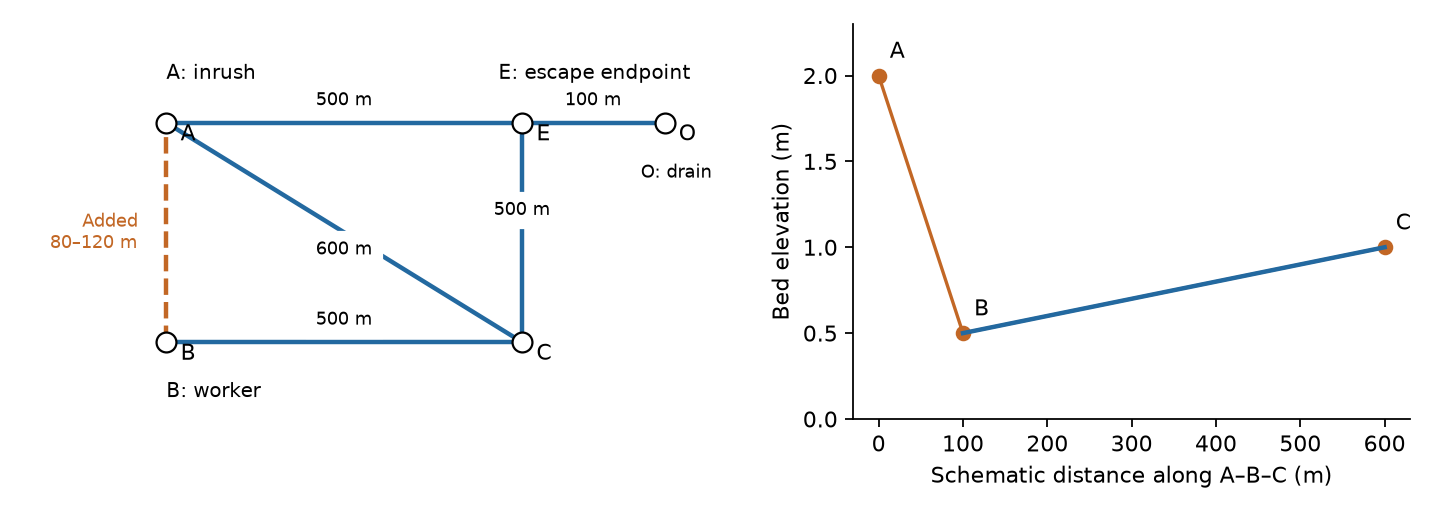
\includegraphics[width=\linewidth]{figures/geometry.png}
\caption{The original network and the dashed added connection. The elevation profile illustrates the representative case; the network drawing is schematic, not a surveyed mine plan.}\label{fig:geometry}
\end{figure}

The original links are \(AE=500\), \(AC=600\), \(BC=500\), \(CE=500\), and \(EO=100\), with lengths in meters. The added link is \(AB\). Elevations are \(z_A=2\), \(z_C=1\), \(z_E=0\), and \(z_O=-0.2\) meters; \(z_B\) varies. Each tunnel has rectangular width \(4\) meters and nominal height \(3\) meters, with a linear floor profile between endpoints. The original shortest walking distance is \(1000\) meters, along \(BCE\). With an 80- or 120-meter connection it becomes 580 or 620 meters, along \(BAE\).

The worker's origin is lower than both \(A\) and \(C\). In the original layout, water can reach that depression only through the longer route via \(C\). Adding \(AB\) creates a more direct downhill supply from the inrush. It also diverts flow away from other branches. These two hydraulic effects act on different timescales. A prompt evacuee can leave the depression before substantial accumulation; a late evacuee starts in the accumulated water.

The dimensions are a controlled hydraulic scenario, not a reconstruction of an accident. The width and central inflow follow the competition setting. The inflow range \(0.4\)--\(0.6\,\mathrm{m^3\,s^{-1}}\) brackets that value. The short-connection grades are approximately \(1.1\%\)--\(2.1\%\); the other links have smaller grades. Manning coefficients \(0.02\)--\(0.03\,\mathrm{s\,m^{-1/3}}\) are sensitivity values of the order used for excavated channels \cite{usda}, not measured coefficients for a particular mine.

We deliberately retain a small topology. It permits complete path enumeration, examination of the water field, and an explicit witness. A large CAD network would add uncertain junctions, interpolated elevations, and unspecified hydraulic outlets before clarifying the mechanism. The numerical evidence here supports a possibility and its cause, not its frequency across operating mines.

\section{Hydraulic calculations and numerical verification}
\subsection{Independent finite-volume calculation}
The main independent calculation solves one-dimensional shallow-water equations in each constant-width tunnel. Let \(h\) be water depth, \(q=hu\) discharge per unit width, \(u\) mean velocity, and \(z\) bed elevation. With gravitational acceleration \(g=9.81\,\mathrm{m\,s^{-2}}\),
\begin{align}
 \partial_t h+\partial_x q&=0,\\
 \partial_t q+\partial_x\!\left(\frac{q^2}{h}+\frac{gh^2}{2}\right)
 &=-gh\,\partial_x z-\frac{g n^2 q|q|}{h R^{4/3}},
 \qquad R=\frac{wh}{w+2h},                               \label{eq:swe}
\end{align}
where \(w\) is width, \(R\) the hydraulic radius, and \(n\) Manning roughness. Dry states use zero discharge.

We use a first-order Harten--Lax--van Leer flux with dry-bed wave-speed bounds and hydrostatic reconstruction following Audusse et al.~\cite{audusse}. Friction is updated semi-implicitly. A Courant factor of \(0.35\), additional local draining limits, and a maximum one-second step preserve nonnegative depths in the network runs. These are established numerical methods; the solver is an independently implemented check, not a proposed new hydrodynamic scheme.

Junctions are finite-area mixed chambers with common water level and no resolved momentum. A chamber of plan area \(S_j\) obeys
\[
 S_j\,\frac{\dd h_j}{\dd t}=Q_j^{\rm source}
       +\sum Q_j^{\rm in}-\sum Q_j^{\rm out}.
\]
The same interface flux updates the adjacent channel and chamber, so internal transfers cancel exactly in the volume balance. The base area is \(16\,\mathrm{m^2}\). This coupling represents a specified storage/mixing idealization; it does not resolve three-dimensional junction circulation or guarantee the correct loss coefficient for an actual intersection. We vary the area rather than conceal that assumption.

The network starts dry. A constant source enters \(A\) at time zero. The downstream boundary is transmissive. No pumping, infiltration, debris, roof collapse, or pressurized flow is included. The modeled depths in the confirmation runs remain below the nominal roof.

\subsection{SWMM comparison}
The second calculation uses the United States Environmental Protection Agency's Storm Water Management Model (SWMM), accessed through \texttt{swmm-toolkit} 0.17.0, with dynamic-wave routing \cite{swmm}. The same links, elevations, cross sections, roughness, and source are supplied, but SWMM uses its own junction and outlet treatment. The source enters a junction and \(O\) is a free outfall. The main factorial uses 6.25-meter maximum segment length, a fixed 0.125-second routing step, and two-second output intervals.

The two calculations are not independent samples from a distribution of true models. They share depth-averaged physics and idealized geometry. Agreement is evidence of robustness to these two implementations and their junction treatments. Disagreement is also evidence and is reported below.

\subsection{Checks that passed, and one that did not}
Mass conservation alone is insufficient to verify flood arrival times. We therefore checked steady flow, an advancing dry-bed front, and network equilibrium separately.

For SWMM, six uniform-flow tests used a 500-meter rectangular channel, prescribed upstream flow, a downstream stage equal to Manning normal depth, and initial uniform depth. These check the interface and a steady solution, not a transient mine inrush.

For the independent finite-volume core, we used Ritter's frictionless dry-bed dam-break solution, a standard shallow-water benchmark \cite{swashes}. With one meter of water initially to the left of \(x=0\), the solution before boundary influence is
\[
 h(x,t)=
 \begin{cases}
 1,&x\leq-\sqrt g\,t,\\
 (2\sqrt g-x/t)^2/(9g),&-\sqrt g\,t<x<2\sqrt g\,t,\\
 0,&x\geq2\sqrt g\,t .
 \end{cases}
\]
At \(t=100\) seconds, mean absolute depth error over \(|x|<700\) meters decreased from \(0.01634\) to \(0.00421\) meters as cell size decreased from 25 to 3.125 meters. Mass residual was at most \(2.3\times10^{-13}\) per unit width. A nonflat lake-at-rest test preserved depth to \(6.7\times10^{-16}\) meters. Network checks preserved a symmetric dry-start fork exactly and a nonflat closed-loop lake at rest; the fork's volume residual was \(7.1\times10^{-15}\,\mathrm{m^3}\).

The analogous SWMM dry-bed test was unsatisfactory. Even with inertial damping disabled, the tested setup at 6.25-meter spacing placed the \(h>0.01\) meter front at 281.25 meters after 100 seconds, versus the analytical \(h=0.01\) meter location of 532.46 meters. Its mean depth error was approximately \(0.0795\) meters. SWMM also issued minimum-elevation-drop warnings for the flat links. This test does not establish that every SWMM configuration fails; initialization and model options matter. It does prevent treating the SWMM results as a validated transient reference. The finite-volume result is the main physically explicit calculation; SWMM is a robustness comparison with a documented limitation.

The finite-volume front also converges more slowly than its integrated depth error: at 3.125-meter spacing its \(h>0.01\) front was 495.31 meters. We therefore do not infer subsecond arrival precision from small volume residuals.

\section{Experiment and trajectory evaluation}
\subsection{Frozen factorial after exploratory discovery}
An exploratory search identified the low-lying-origin mechanism. We then wrote a local protocol before running new parameter combinations:
\[
 Q\in\{0.4,0.6\},\quad n\in\{0.02,0.03\},\quad
 z_B\in\{0.3,0.7\},\quad L_{AB}\in\{80,120\}.
\]
The resulting \(2^4=16\) cases were each run with and without the connection under both hydraulic models, giving 64 calculations. The protocol and its SHA-256 digest were saved before execution. This was a frozen follow-up to adaptive discovery, not external preregistration or a representative sample of mines.

The primary prediction required both
\begin{equation}
 E_1^{\rm sp}(0)-E_0^{\rm sp}(0)\leq-0.02\ {\rm m},
 \qquad
 E_1^{\rm sp}(600)-E_0^{\rm sp}(600)\geq0.02\ {\rm m}       \label{eq:criterion}
\end{equation}
in \emph{both} models. The 2\,cm threshold is a prespecified materiality margin for this numerical comparison, not a medical threshold. We report every case, including misses.

Numerical gates required finite values, nonnegative depths, no roof exceedance, SWMM continuity error below \(1\%\), no reported SWMM flooding loss or nonconverging steps, and finite-volume mass residual below \(10^{-6}\,\mathrm{m^3}\). These gates catch implementation failures; they do not replace the benchmark tests or establish field calibration.

\subsection{Route envelopes and continuous witness peaks}
The path comparison interpolates the saved depth field in space and time, permits depth to recede, and does not permanently close a tunnel at its first threshold crossing. The main factorial samples trajectories at intervals of at most one second. It includes the origin, all segment endpoints, and arrival. Departure-grid results elsewhere use two-second increments and explicitly censor arrivals beyond the one-hour horizon.

For the certificate, we removed trajectory sampling error relative to the saved reconstruction. In one space--time cell, bilinear depth interpolation composed with constant-speed motion is a quadratic function of time. Split the trajectory whenever it crosses a spatial knot or an output time. On each resulting interval, evaluate both endpoints and any interior concave quadratic vertex. Taking their maximum gives the exact peak for that reconstruction, up to floating-point arithmetic.

This calculation is exact for interpolated output, not for the unknown continuum hydraulic solution. The distinction matters: spatial refinement and hydraulic time-step checks remain necessary. We verified the evaluator on a field \(h(x,t)=x(1-t)\), whose trajectory \(x=t\) has the interior maximum \(1/4\), and on its reverse traversal.

The old-layout witness is always \(BCE\). At departure \(d=600\) seconds we evaluate it at speeds \(0.7,1.0,1.3\,\mathrm{m\,s^{-1}}\), then compare its peak to \(h_1(B,600)\). This post-hoc mechanism analysis is separate from the frozen primary prediction.

\section{Results}
\subsection{The benefit changes sign with delay}
Figure~\ref{fig:curve} shows a representative exploratory case with \(Q=0.5\,\mathrm{m^3\,s^{-1}}\), \(n=0.025\), \(z_B=0.5\) meters, and \(L_{AB}=100\) meters. The two models disagree on the exact crossover time and depths, but both show the same reversal.

\begin{figure}[htbp]
\centering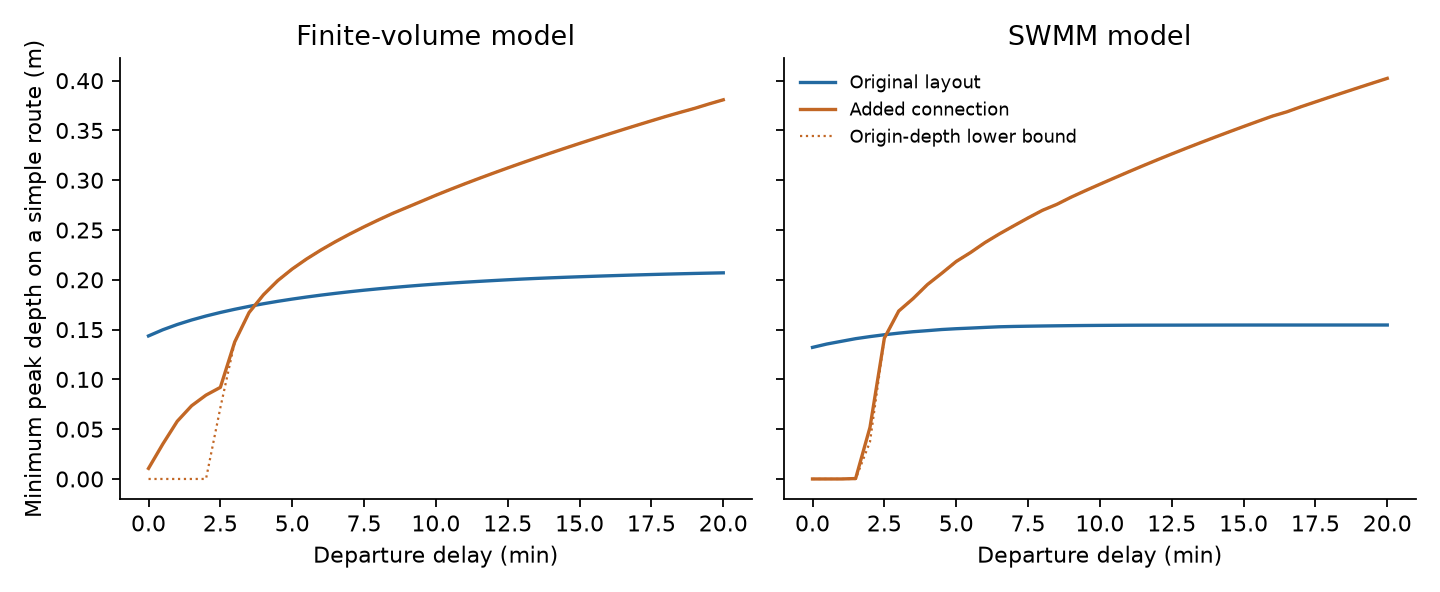
\includegraphics[width=\linewidth]{figures/delay_curve.png}
\caption{Best simple-route peak depth versus departure delay in the representative case. The dotted origin-depth lower bound eventually coincides with the added-layout envelope.}\label{fig:curve}
\end{figure}

For immediate departure, finite-volume peak exposure decreases from approximately \(0.144\) to \(0.011\) meters; SWMM decreases from \(0.132\) to zero. At a ten-minute delay, the finite-volume comparison is \(0.196\) versus \(0.285\) meters, and SWMM is \(0.154\) versus \(0.296\) meters. At twenty minutes, the corresponding comparisons are approximately \(0.207\) versus \(0.381\), and \(0.155\) versus \(0.402\) meters.

The early improvement should not be attributed automatically to walking along the shortcut. In the confirmation factorial, \(BCE\), an old route, is early peak-depth optimal in all 16 added-layout finite-volume cases and 15 of 16 SWMM cases. The connection changes the water field enough to improve an existing route. As water accumulates at \(B\), that hydraulic advantage reverses. This separates a hydraulic mechanism from a claim about a superior path-search algorithm.

\subsection{Confirmation, including the misses}
Twelve of the 16 new parameter combinations satisfy \eqref{eq:criterion} in both models (Figure~\ref{fig:confirmation}). Cases 4--7 fail the primary criterion because SWMM's early improvement is about \(1.98\) centimeters, just below the frozen 2\,cm cutoff. They are not rounded into successes. All 16 show late deterioration of at least 2\,cm in both models.

\begin{figure}[htbp]
\centering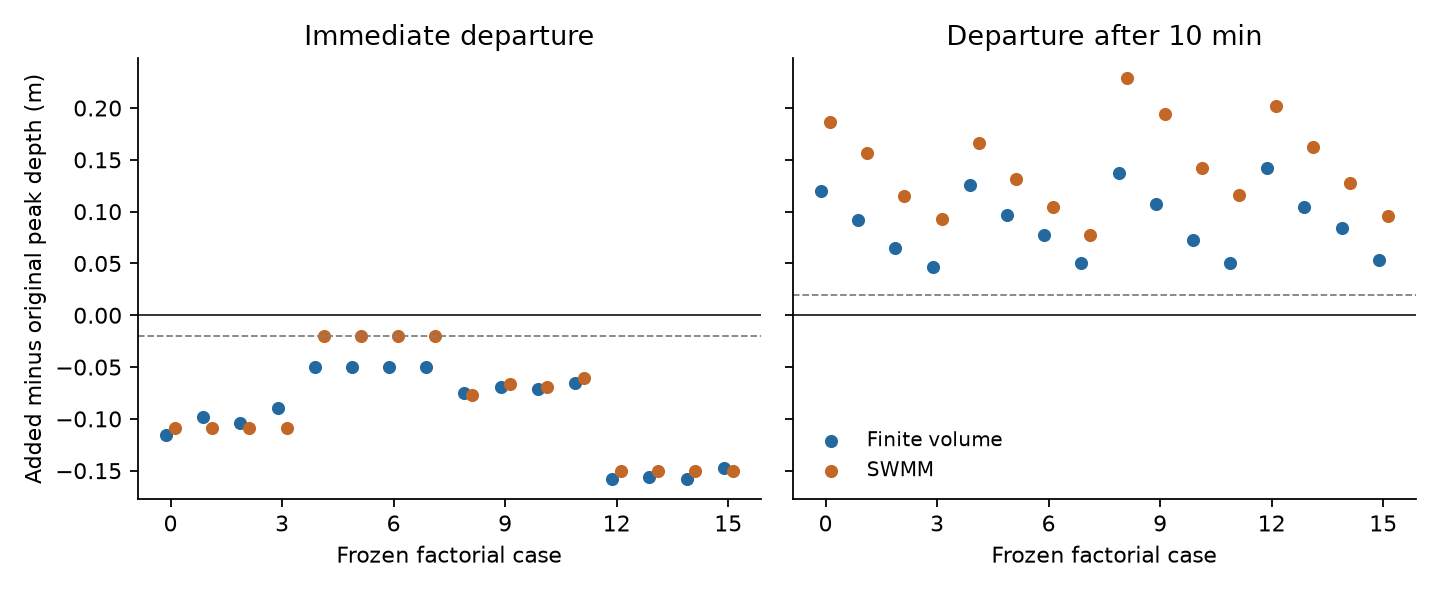
\includegraphics[width=\linewidth]{figures/confirmation.png}
\caption{All 16 frozen cases. Negative values favor the added connection; dashed lines mark the prespecified 2\,cm margins. Case indices follow lexicographic order of \(Q,n,z_B,L_{AB}\).}\label{fig:confirmation}
\end{figure}

All confirmation runs pass the numerical gates. The largest absolute SWMM global continuity error is \(0.072\%\); the largest finite-volume absolute volume residual is \(2.1\times10^{-11}\,\mathrm{m^3}\). These small residuals establish accounting consistency, not precise arrival-time prediction.

The continuous certificate is positive in all 96 combinations of 16 cases, two models, and three witness speeds. Its smallest margin is \(0.0350\) meters. Thus the late loss is not explained by restricting the new-layout route search to simple paths: even an unrestricted new-layout policy must incur the origin depth. The old-layout origin remains dry up to 600 seconds in all confirmation outputs, so including predeparture waiting exposure does not increase the old witness bound. The count of 96 is a collection of designed checks with shared inputs, not 96 statistically independent observations.

\subsection{Refinement and junction storage}
We refined three cases: the first factorial corner (0), a weak early-benefit case (7), and the smallest late-certificate case (15). The finite-volume calculation used 3.125- and 1.5625-meter cells; SWMM used 3.125-meter segments and a 0.0625-second routing step. Table~\ref{tab:refinement} reports the certificate for the slowest constant-speed witness, \(0.7\,\mathrm{m\,s^{-1}}\).

\begin{table}[htbp]\centering
\caption{Late certificate margins, in centimeters. All signs persist; the values are not claimed to be fully converged.}\label{tab:refinement}
\begin{tabular}{lrrr}\toprule
Calculation & Case 0 & Case 7 & Case 15\\\midrule
Finite volume, 3.125 m &10.44&3.13&3.21\\
Finite volume, 1.5625 m&9.76&2.84&2.95\\
SWMM, 3.125 m&18.73&7.44&9.37\\\bottomrule
\end{tabular}
\end{table}

For case 15, the finite-volume margin decreases from \(3.50\) centimeters at 6.25-meter spacing to \(2.95\) centimeters at 1.5625-meter spacing. The sign survives, but the trend precludes presenting the coarser number as exact.

Changing the mixed-chamber area from \(16\) to \(4\) or \(64\,\mathrm{m^2}\), at 3.125-meter spacing in case 15, gives margins of \(3.52\) and \(1.93\) centimeters. Larger storage weakens the effect. The latter remains positive but falls below the original 2\,cm materiality criterion; not every expanded sensitivity passes that threshold.

\subsection{Depth-responsive walking and model disagreement}
Constant speed could favor a witness that becomes implausibly fast in water. We therefore evaluated two additional witness policies. At each one-meter spatial step, the worker sets
\[
 v=\frac{1\,\mathrm{m\,s^{-1}}}{1+k h_{\rm current}},
 \qquad k\in\{2,4\}\,\mathrm{m^{-1}},
\]
and holds that speed to the next step. These are stress-test laws, not fitted gait models. Each step is a linear trajectory, so its reconstructed-field peak can still be evaluated continuously. All 64 checks finish within the simulation horizon and retain a positive certificate; the minimum margin is \(0.0460\) meters.

The models do not agree universally. An earlier matched sweep used seven flows from \(0.5\) to \(2.0\,\mathrm{m^3\,s^{-1}}\), with a fixed low origin, and gives different classifications under a 0.3-meter closure threshold. Both models show harm at flows \(0.5\), \(0.8\), and \(1.0\), disagree at \(1.2\) and \(1.4\), and provide a feasible sampled route only after adding the connection at \(1.6\) and \(2.0\), in the same flow units. At \(Q=1.4\), the finite-volume model finds no old-layout route below 0.3 meters, whereas SWMM does. These findings rule out a universal claim that added connections worsen escape.

They also motivate the exposure comparison and certificate: a single binary safety threshold can hide both the magnitude of disagreement and the reason for a route's failure. The favorable confirmation result is local to its stated parameter family.

\section{Interpretation and limitations}
The result is a failure of fixed-hazard network intuition. On a graph with unchanged edge conditions, an extra option cannot worsen an optimal route. Here the added connection changes the conditions on existing routes and at the origin. Early diversion and later accumulation can have opposite effects even when the worker uses the same escape path.

This does not imply that removing mine connections is a safety strategy. Cross passages can be indispensable for other inrush locations, fires, ventilation, rescue access, and congestion. Nor does the experiment optimize a door-closing schedule or establish that a water barrier can be operated safely. It identifies a quantity that a layout assessment should examine: whether a connection's hydraulic effect raises origin exposure during a plausible response delay.

Several boundaries are substantial.
\begin{enumerate}
\item \textbf{No field calibration.} The geometry is idealized, the inflow is prescribed, and the junction treatments are approximations. Neither model is validated against measurements of the proposed motif or an operating mine. The credible component is the stated conservation-law model and its numerical checks; the study does not establish predictive accuracy at a site.
\item \textbf{Depth is not complete hazard.} Velocity and human stability are omitted from the objective. A lower peak depth need not mean a safer journey if the current is faster. The conclusion is specifically about depth exposure.
\item \textbf{A local network family.} All confirmation cases share a low-lying origin and one topology. They establish persistence under several parameter changes, not prevalence across mine layouts. Large junction storage and alternative drainage may mitigate or remove the effect.
\item \textbf{Numerical uncertainty remains.} The certificate is exact only for reconstructed outputs. Refinement preserves its sign in selected cases but does not supply a rigorous PDE error bound. SWMM's dry-front discrepancy and the models' threshold disagreements are material qualifications.
\item \textbf{The early comparison has a restricted policy class.} It enumerates simple paths at a fixed speed. The late certificate has broader scope, but it still prescribes the worker's location and departure time. Advance relocation and a different warning policy change the problem.
\end{enumerate}

The practical lesson is therefore methodological: evaluate the hydraulic and evacuation effects of an added connection together, and report the departure regime. A shorter dry route and an early favorable simulation do not settle the late-evacuation comparison.

\section{Conclusion}
An added tunnel can initially shield an escape route by diverting water, then increase unavoidable exposure by supplying the worker's low-lying origin. The tested reversal survives two hydraulic treatments and a frozen parameter study, while its magnitude and some threshold classifications remain model dependent.

The next question is whether the origin-depth certificate can guide selective, field-informed analysis of larger networks. Candidate connections could first be screened for short hydraulic access to occupied depressions, then checked with measured junction geometry and transient observations. A second question is whether detection, relocation, or controlled hydraulic isolation can preserve early benefits without creating late accumulation. Answering either requires information beyond a dry connectivity map.

\appendix
\section{Reproducibility and scope of the research record}
The accompanying local research package contains all inputs, code, hydraulic output, and negative findings. The original competition work and earlier manuscript are preserved separately. The new computation is organized as follows:
\begin{itemize}
\item \texttt{shallow\_water.py} and \texttt{network\_fv.py}: independent finite-volume implementation and its checks.
\item \texttt{benchmark\_swmm.py}, \texttt{benchmark\_transient.py}, and \texttt{shortcut\_screen.py}: SWMM verification and synthetic networks.
\item \texttt{confirmation\_protocol.json} and \texttt{run\_confirmation.py}: frozen conditions and the full factorial.
\item \texttt{continuous\_certificate.py}, \texttt{refine\_confirmation.py}, and \texttt{slowed\_witness.py}: continuous reconstructed-field evaluation and sensitivity checks.
\end{itemize}
The principal result files are:
\begin{quote}\small\ttfamily
confirmation\_v1/results.json\\
confirmation\_v1/audit.json\\
confirmation\_v1/continuous\_certificate.json\\
confirmation\_refinement/results.json
\end{quote}
Figure generation uses retained results rather than rerunning selected successes.

The original exploratory search and the later confirmation are intentionally distinguished. Exploratory variants include higher flows, alternative depth thresholds, and an earlier simplified volume-transfer model. Those variants were not used as an independent test set. The confirmation was frozen only after the candidate mechanism was identified.

No surveyed CAD drawing is required to reproduce this paper. No real accident, field validation, author identity, affiliation, or publication status is inferred from the numerical record. The implementation, mathematical development, and manuscript were prepared with AI assistance; human authorship review and responsibility are required before external circulation.

\begin{thebibliography}{9}\small
\bibitem{wu}
Q. Wu et al. Finding the earliest arrival path through a time-varying network for evacuation planning of mine water inrush. \emph{Safety Science} 130 (2020), 104836.
\href{https://doi.org/10.1016/j.ssci.2020.104836}{doi:10.1016/j.ssci.2020.104836}.
\bibitem{pan}
D. Pan, S. Tai, W. Xu, Y. Du, H. Chen, and A. Hu.
Volume of Fluid Implementation of Water Inrush and Escape Route Optimization in Tunnel.
\emph{Periodica Polytechnica Civil Engineering} 69(3) (2025), 850--868.
\href{https://doi.org/10.3311/PPci.39878}{doi:10.3311/PPci.39878}.
\bibitem{cumcm}
China Society for Industrial and Applied Mathematics.
\emph{CUMCM 2025, Problem D: Mine water-inrush propagation and escape planning}.
Supplied problem statement and attachments; competition information:
\url{https://en.mcm.edu.cn/}.
\bibitem{usda}
USDA Agricultural Research Service.
\emph{WEPP User Summary}, channel roughness tables.
\url{https://www.ars.usda.gov/ARSUserFiles/50201000/WEPP/usersum.pdf}.
\bibitem{audusse}
E. Audusse, F. Bouchut, M.-O. Bristeau, R. Klein, and B. Perthame.
A fast and stable well-balanced scheme with hydrostatic reconstruction for shallow water flows.
\emph{SIAM Journal on Scientific Computing} 25(6) (2004), 2050--2065.
\href{https://doi.org/10.1137/S1064827503431090}{doi:10.1137/S1064827503431090}.
\bibitem{swmm}
US Environmental Protection Agency.
\emph{Storm Water Management Model User's Manual, Version 5.2}.
EPA/600/R-22/030, February 2022.
\href{https://www.epa.gov/system/files/documents/2022-02/storm-water-management-model-users-manual-version-5.2.pdf}{Official manual}.
\bibitem{swashes}
O. Delestre et al.
SWASHES: a compilation of shallow water analytic solutions for hydraulic and environmental studies.
\emph{International Journal for Numerical Methods in Fluids} 72(3) (2013), 269--300.
\href{https://doi.org/10.1002/fld.3741}{doi:10.1002/fld.3741}.
\end{thebibliography}
\end{document}
